\section{Neural Networks}
\subsection{Model Implementation}
In this project, we implemented the neural network model using PyTorch’s nn.Module. The NeuralNetworkModel class is built to predict customer churn from the Telco dataset. The model starts with an input layer that takes in 26 features (which corresponds to the number of features in the dataset) and maps them to a specified number of hidden neurons, with the default being 15 neurons. This number can be adjusted depending on the model's complexity. The model also allows for flexibility in the number of hidden layers, which can be defined by the num\_hidden\_layers parameter. Each hidden layer consists of a fully connected layer followed by a ReLU activation function, which adds non-linearity to the network and allows it to learn more complex relationships. To prevent overfitting, we include a dropout layer after each hidden layer, with a 50\% probability by default. This means that during training, half of the neurons are randomly set to zero, forcing the model to generalize better.\\

The output layer consists of a single neuron that is connected to the last hidden layer. This output is passed through a Sigmoid activation function, which compresses the result into a value between 0 and 1. This output represents the probability of a customer churning. The forward method defines how the data flows through the network: it starts at the input layer, passes through the hidden layers with ReLU activations, and ends at the output layer with the Sigmoid function applied. This design enables the model to capture complex patterns in customer behavior while controlling for overfitting using dropout. The model is structured as a sequential model, making it easy to define and implement multiple layers in a straightforward manner.

\subsection{Training Implementation}
The train function is responsible for training the neural network model. It starts by initializing the model using the NeuralNetworkModel class, setting parameters like the input size, hidden layer size, number of hidden layers, and dropout rate. The function then creates data loaders for both the training and validation datasets, allowing the data to be processed in batches, which helps manage memory usage and speeds up training.\\

For the loss function, Binary Cross-Entropy Loss (BCELoss) is used, as it is well-suited for binary classification problems, such as predicting whether a customer will churn. The Adam optimizer is chosen because it efficiently adjusts the learning rate based on gradients, making the training process faster and more stable.\\

The training loop runs for a set number of epochs, with each epoch representing one full pass through the training data. During each epoch, the model is put in training mode, and the optimizer gradients are reset to zero before processing each batch. The input data is passed through the model, and the loss is calculated by comparing the model’s predictions with the actual labels. The loss is then backpropagated through the network to compute gradients, and the optimizer updates the model's weights accordingly.\\

At the end of each epoch, the average training loss is calculated and saved for later analysis. Afterward, the model is evaluated on the validation dataset, using the same process but in evaluation mode (with no gradient calculation). The validation loss is also calculated and tracked. Every 10 epochs, the training and validation losses are printed to help monitor the model's progress.\\

Once all epochs are completed, the function returns the trained model along with the lists of training and validation losses. These losses can be used to evaluate the model's performance and see how it improves over time. Overall, this implementation provides a structured approach to training and evaluating the neural network while keeping track of its progress at each step.

\subsection{Model Tuning Implementation}
The tune\_hyperparameters function is used to optimize the hyperparameters of the neural network model with the help of Optuna, a framework for hyperparameter optimization. It accepts several inputs: the training function (model\_train\_fn), training and validation data (X\_train, y\_train, X\_val, y\_val), the number of trials for optimization (n\_trials), the optimization direction (either minimize or maximize), and the search space for the hyperparameters.\\

 The function starts by setting up an Optuna study, specifying the direction of optimization and using a TPESampler to guide the search. Then, the optimization process begins, and for each trial, it calls the model\_train\_fn function, passing the training and validation data, along with the current trial's hyperparameters. Once all the trials are complete, the function logs the best set of hyperparameters found during the search process. It then returns the Optuna study object, which holds details about the entire optimization process. This approach allows for efficient hyperparameter tuning, helping to find the best configuration for the neural network to improve its performance.

\subsection{Training Process}
The training process begins by training the neural network model using manually selected hyperparameters. In this initial step, we set key hyperparameters such as the hidden layer size, number of hidden layers, dropout rate, learning rate, weight decay, batch size, and the number of epochs. These parameters are passed into the train\_and\_save function, which trains the model according to the given settings and saves both the model and training results.\\

After completing the initial training, we move on to fine-tuning the model by optimizing its hyperparameters. We define a search space that includes a range of values for hyperparameters such as learning rate, batch size, hidden layer size, number of hidden layers, dropout rate, epochs, and weight decay. We use the tune\_and\_save function to run 50 trials, with the goal of minimizing the validation loss and finding the best combination of hyperparameters. After the tuning process is finished, the best hyperparameters are selected.\\

Finally, with the optimal hyperparameters identified, we re-train the model using the train\_study\_and\_save function, ensuring that the model is trained with the most effective settings. Once training is complete, the model and its results are saved for further evaluation and deployment. This process ensures that the model is not only trained with appropriate hyperparameters but also optimized for better performance.

\subsection{Manual Training Results and Analysis}

\begin{figure}[hbt!]
    \centering
    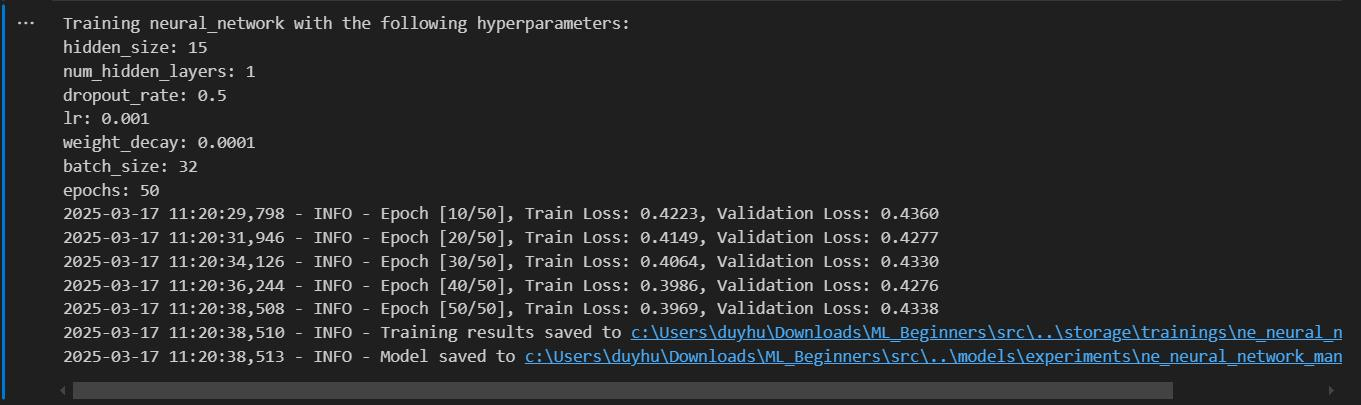
\includegraphics[width=1\linewidth]{Images/5.5.a.jpg}
    \caption{Training Log for Manual Hyperparameters }
    \label{fig:enter-label}
\end{figure}

In this step, the neural network model is trained with manually selected hyperparameters. The training runs for 50 epochs, with key hyperparameters such as a hidden layer size of 15 neurons, one hidden layer, dropout rate of 0.5, learning rate of 0.001, weight decay of 0.0001, batch size of 32, and a total of 50 epochs. The training and validation losses show that the model improves over time, but the validation loss remains relatively stable by the end of the training, indicating that there may still be room for improvement, particularly in generalizing to unseen data.
\subsubsection{Evaluation and Cross-Validation}

\begin{figure}[hbt!]
    \centering
    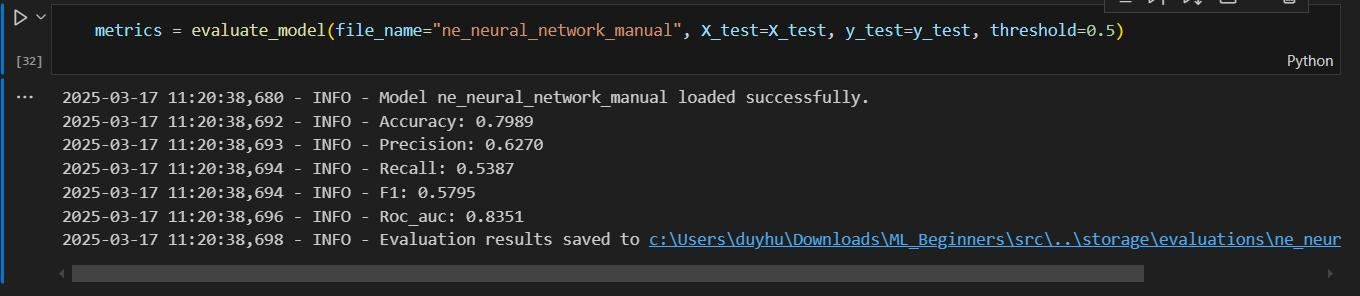
\includegraphics[width=1\linewidth]{Images/5.5.1.a.jpg}
    \caption{Model Evaluation and Cross-Validation Results for Manual Hyperparameters}
    \label{fig:enter-label}
\end{figure}

The model evaluation shows decent performance with an accuracy of 79.89\%, meaning the model correctly predicted churn about 80\% of the time. The precision score of 0.6270 suggests that when the model predicts churn, it is accurate 63\% of the time, but the recall of 0.5387 indicates it misses around 46\% of the actual churn cases. This demonstrates that the model is conservative in predicting churn and misses a significant portion of churners. The F1 score of 0.5795 reflects a balance between precision and recall, but the model could improve in identifying more churn cases. The ROC AUC score of 0.8351 suggests that the model can effectively distinguish between churn and non-churn customers, but there’s still room for improvement.\\

When evaluated using cross-validation, the model shows similar metrics, with a slight improvement in precision (0.6628) and accuracy (0.7996). However, the recall remains low at 0.5015, highlighting that the model is still missing a considerable number of churn cases. The F1 score of 0.5707 and ROC AUC score of 0.8378 further confirm that while the model performs well, improving recall remains a key area for development to capture more churn cases.

\subsubsection{Loss Curves}

\begin{figure}[hbt!]
    \centering
    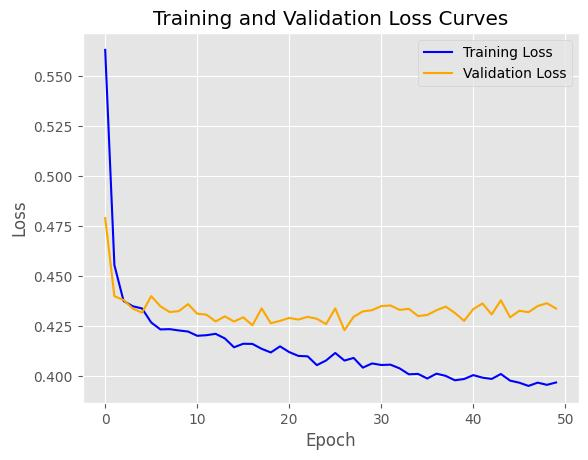
\includegraphics[width=1\linewidth]{Images/5.5.2.a.jpg}
    \caption{Training and Validation Loss Curves for Manual Hyperparameters}
    \label{fig:enter-label}
\end{figure}

The loss curve shows a sharp initial drop in both training loss and validation loss, indicating that the model is quickly learning. However, the training loss decreases faster than the validation loss, suggesting that the model fits the training data well but struggles to generalize to unseen data. As training continues, both losses stabilize, but the training loss remains lower than the validation loss, which is a sign of potential overfitting. This could be improved with techniques like regularization or early stopping to help the model generalize better to new data.

\subsubsection{Confusion Matrix}

\begin{figure}[hbt!]
    \centering
    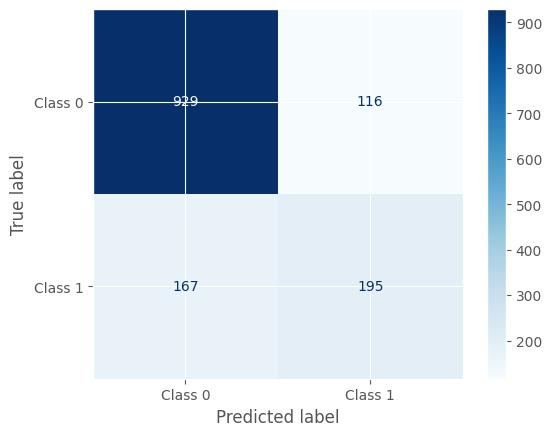
\includegraphics[width=1\linewidth]{Images/5.5.3.a.jpg}
    \caption{Confusion Matrix for Manual Hyperparameters}
    \label{fig:enter-label}
\end{figure}

The confusion matrix reveals that the model performs well in predicting non-churning customers, correctly predicting 919 true negatives and 195 true positives. However, the model makes 116 false positives and 167 false negatives, meaning it incorrectly predicts churn for some customers who do not churn and misses many actual churn cases. To improve the model, focusing on reducing false negatives is essential to ensure better accuracy in predicting churn.

\subsubsection{ROC Curve and AUC Score}

\begin{figure}[hbt!]
    \centering
    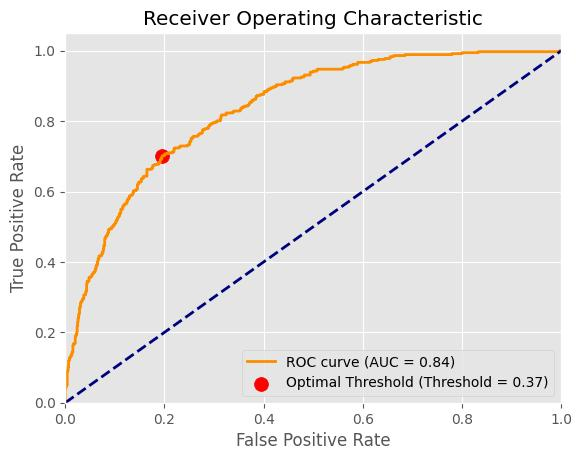
\includegraphics[width=1\linewidth]{Images/5.5.4.a.jpg}
    \caption{ROC Curve for Manual Hyperparameters}
    \label{fig:enter-label}
\end{figure}

The ROC curve indicates that the model is effective at distinguishing between churned and non-churned customers, with an AUC score of 0.84. This is a strong result, suggesting the model can differentiate well between the two classes. The optimal threshold for predicting churn is set at 0.37, which helps balance sensitivity (recall) and specificity (precision). The curve’s distance from the diagonal line shows that the model performs much better than random guessing, confirming that the model is effectively identifying churn cases.

\subsubsection{Precision-Recall Curve}

\begin{figure}[hbt!]
    \centering
    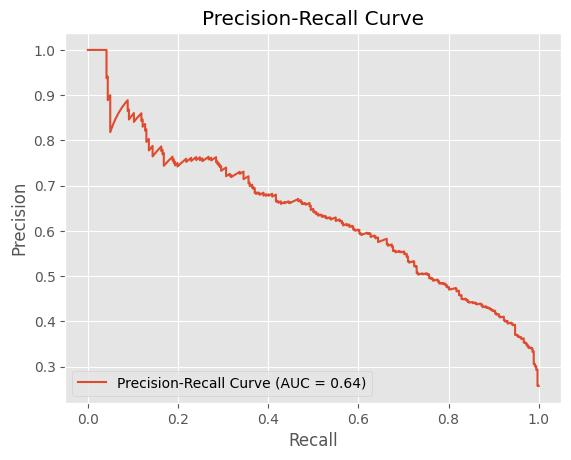
\includegraphics[width=1\linewidth]{Images/5.5.5.a.jpg}
    \caption{Precision-Recall Curve for Manual Hyperparameters}
    \label{fig:enter-label}
\end{figure}

The Precision-Recall curve shows that as recall increases, precision decreases, indicating that the model is trading off precision for recall to identify more churn cases. This is a typical trade-off, where trying to identify more churned customers increases false positives, which lowers precision. The AUC of 0.64 reflects a moderate ability to balance precision and recall, but there’s still room for improvement. Reducing false positives and improving recall would help the model perform better in capturing churn cases.

\subsection{Model Tuning Results and Analysis}

\begin{figure}[hbt!]
    \centering
    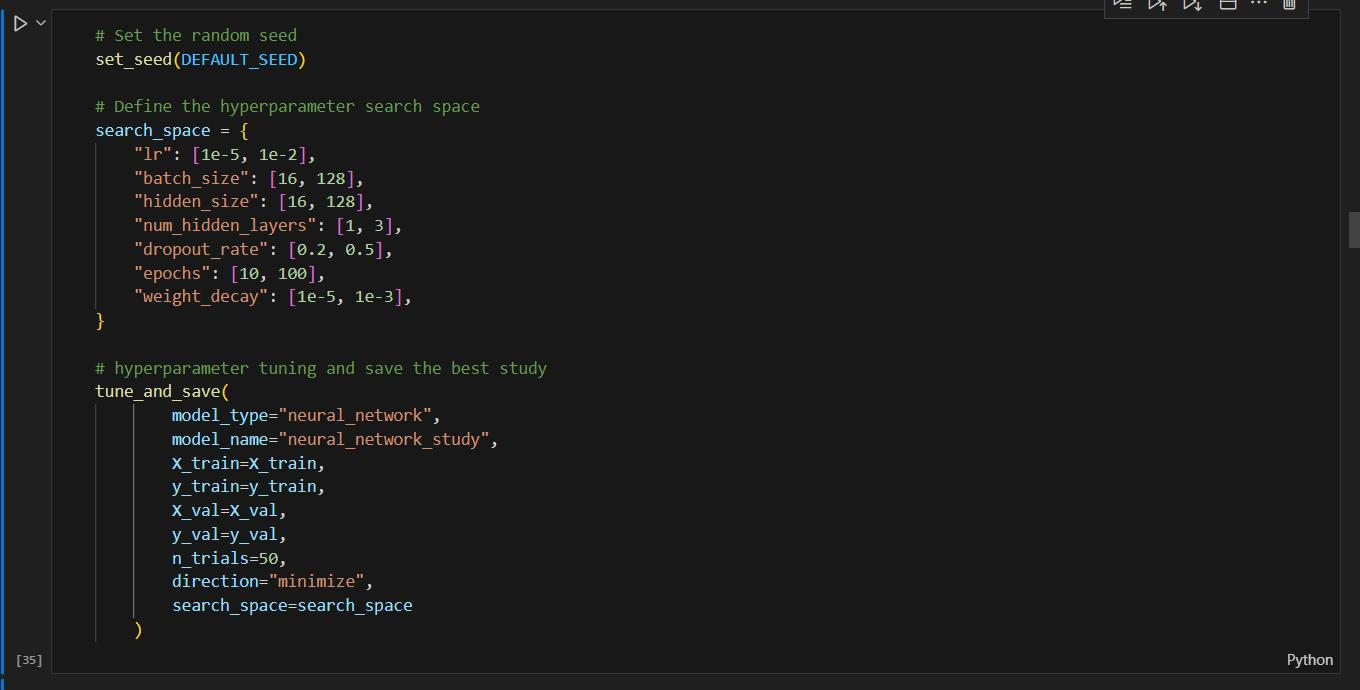
\includegraphics[width=1\linewidth]{Images/5.6.a.jpg}
    \caption{Model Tuning Using Optuna }
    \label{fig:enter-label}
\end{figure}

The hyperparameter tuning for the neural network model was conducted using Optuna to find the best combination of hyperparameters. After defining a search space for hyperparameters such as learning rate, batch size, hidden layer size, number of hidden layers, dropout rate, epochs, and weight decay, Optuna ran 50 trials to minimize the validation loss. The best-performing hyperparameters were a learning rate of 0.00062, a batch size of 94, 94 hidden neurons, 1 hidden layer, a dropout rate of 0.316, 23 epochs, and a weight decay of 0.000898. These optimized settings are expected to improve the model's ability to predict churn more accurately.

\subsubsection{Optimization History Plot}

\begin{figure}[hbt!]
    \centering
    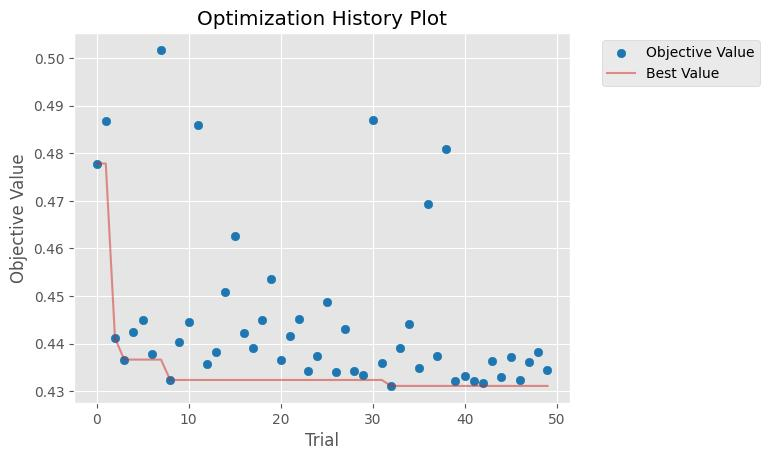
\includegraphics[width=1\linewidth]{Images/5.6.1.a.jpg}
    \caption{Optimization History Plot}
    \label{fig:enter-label}
\end{figure}

The optimization history plot shows how the tuning process unfolded across 50 trials. Early in the process, there is a sharp drop in the objective value, indicating that initial hyperparameter choices made significant improvements to the model. After this initial drop, the objective value stabilizes, and later trials show minimal changes, suggesting the optimization process quickly converged to a good set of hyperparameters. The red line representing the best objective value remains stable after the initial improvement, confirming that the best hyperparameters were found early in the process. This plot demonstrates that the tuning process was both efficient and effective.

\subsubsection{Slice Plot}

\begin{figure}[hbt!]
    \centering
    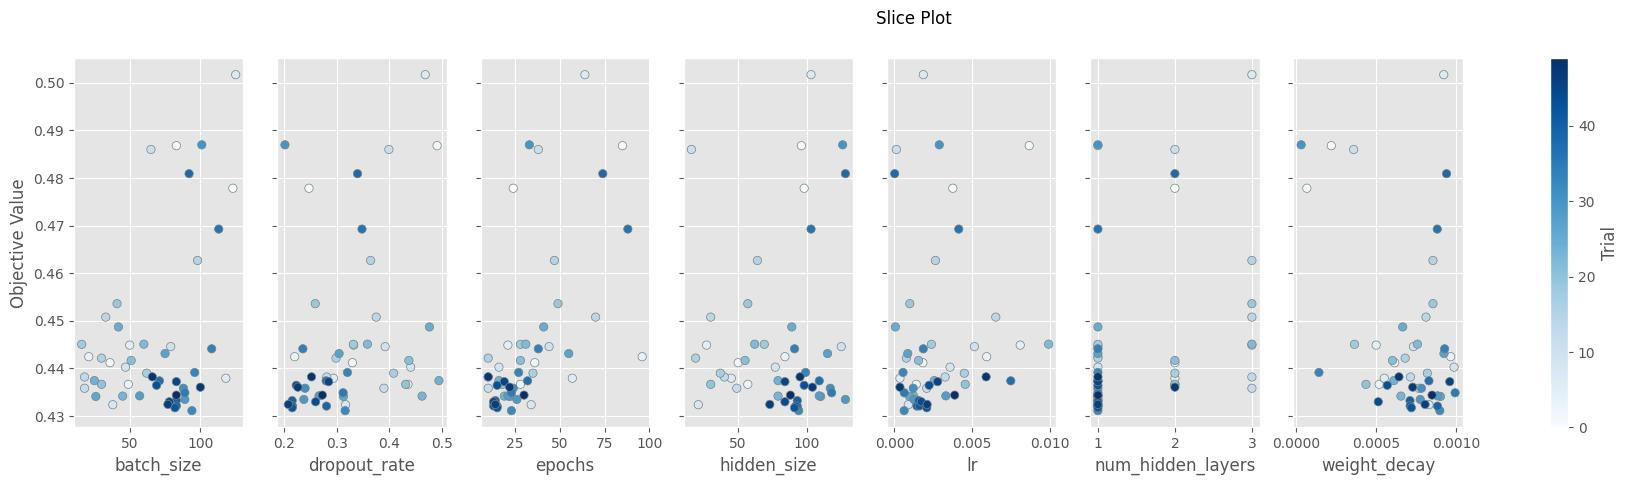
\includegraphics[width=1\linewidth]{Images/5.6.2.a.jpg}
    \caption{Slice Plot}
    \label{fig:enter-label}
\end{figure}

The slice plot illustrates the impact of different hyperparameters on the model's performance. The batch size does not seem to have a strong influence, as the performance is spread evenly across the range. The dropout rate shows some fluctuations, but no clear pattern emerges, suggesting it doesn’t significantly improve model performance. The number of epochs is more impactful, with moderate numbers of epochs leading to better results. The hidden size has a noticeable effect on performance, especially for values between 50 and 100, while the learning rate also plays a significant role, with lower rates yielding better results. The number of hidden layers appears to have a minimal effect, and weight decay shows little variation, indicating it has a smaller impact on the overall model performance. The most influential hyperparameters for improving model performance were learning rate and hidden size, while batch size and dropout rate had a lesser effect.

\subsubsection{Hyperparameter Importances}

\begin{figure}[hbt!]
    \centering
    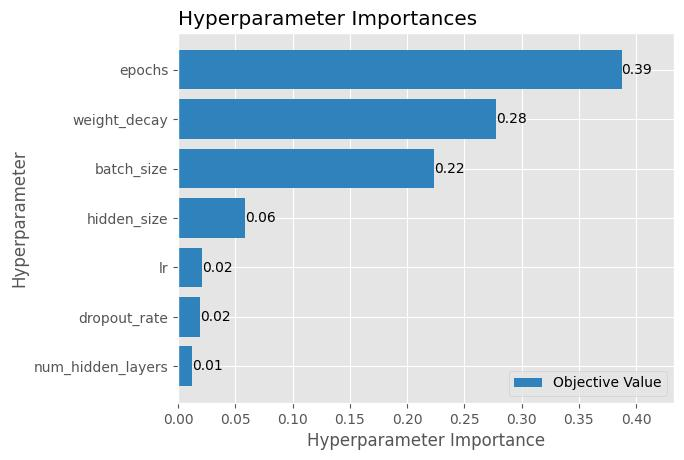
\includegraphics[width=1\linewidth]{Images/5.6.3.a.jpg}
    \caption{Hyperparameter Importances Plot}
    \label{fig:enter-label}
\end{figure}

The hyperparameter importance plot shows that epochs have the highest importance score (0.39), suggesting that the number of epochs is crucial for the model’s ability to learn and generalize effectively. Weight decay (0.28) also plays a significant role in preventing overfitting, while batch size (0.22) impacts the model’s training efficiency and generalization ability. Hidden size has a lower importance score (0.06), showing that the number of neurons in the hidden layers is less significant compared to other hyperparameters. Both learning rate and dropout rate have low importance scores (0.02), suggesting that adjusting these parameters does not lead to substantial improvements in performance. Finally, the number of hidden layers (0.01) has the least impact, indicating that the depth of the model does not significantly affect performance. Overall, the plot suggests that tuning epochs, weight decay, and batch size would yield the most significant improvements in model performance, while other parameters have a smaller impact.

\subsection{Optimal Training Results and Analysis}

\begin{figure}[hbt!]
    \centering
    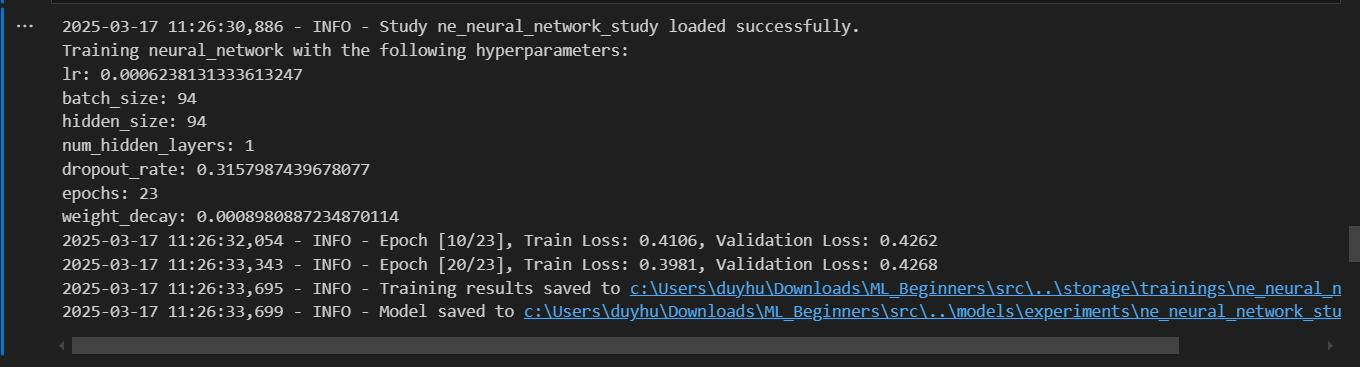
\includegraphics[width=1\linewidth]{Images/5.7.a.jpg}
    \caption{Training Log for Optimal Hyperparameters}
    \label{fig:enter-label}
\end{figure}

The model was trained using the best hyperparameters identified through Optuna. After 10 epochs, the training loss was 0.4106, and the validation loss was 0.4262. By epoch 20, the training loss decreased to 0.3981, while the validation loss remained nearly constant at 0.4268. This suggests that the model is learning over time, but the validation loss isn't improving much, indicating that the model might be nearing convergence. After completing the training, the model and its results were saved for further evaluation.

\subsubsection{Evaluation and Cross-Validation}

\begin{figure}[hbt!]
    \centering
    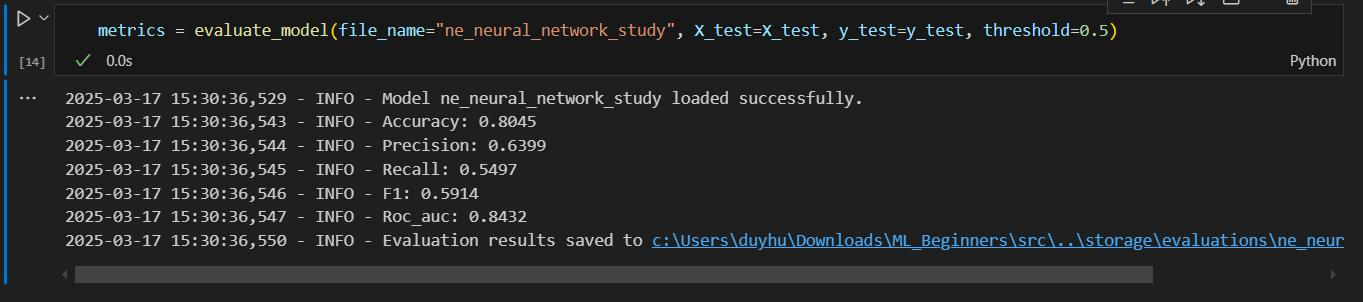
\includegraphics[width=1\linewidth]{Images/5.7.1.a.jpg}
    \caption{Model Evaluation and Cross-Validation Results for Optimal Hyperparameters}
    \label{fig:enter-label}
\end{figure}

When evaluated on the test dataset, the model performed well with an accuracy of 80.45\%. Precision was 0.6399, indicating the model correctly predicts churn 64\% of the time when it makes a churn prediction. The recall was 0.5497, meaning the model identifies about 55\% of actual churn cases but misses a considerable portion. The F1 score was 0.5914, balancing precision and recall, suggesting reasonable performance but with room for improvement, particularly in recall. The ROC AUC score of 0.8432 shows that the model is good at distinguishing between churned and non-churned customers. These metrics indicate solid performance, though improving recall would capture more churn cases.\\

Cross-validation results show an average accuracy of 0.8008, closely matching the test set evaluation. Precision improved slightly to 0.6584, indicating the model is more reliable when predicting churn across multiple folds. However, recall still remains at 0.5190, meaning the model still misses many churned customers. The F1 score was 0.5795, showing a moderate trade-off between precision and recall. The ROC AUC was 0.8426, confirming that the model remains strong in distinguishing churn from non-churn cases. These results suggest the model performs well but still needs further tuning, especially to improve recall.

\subsubsection{Loss Curves}

\begin{figure}[hbt!]
    \centering
    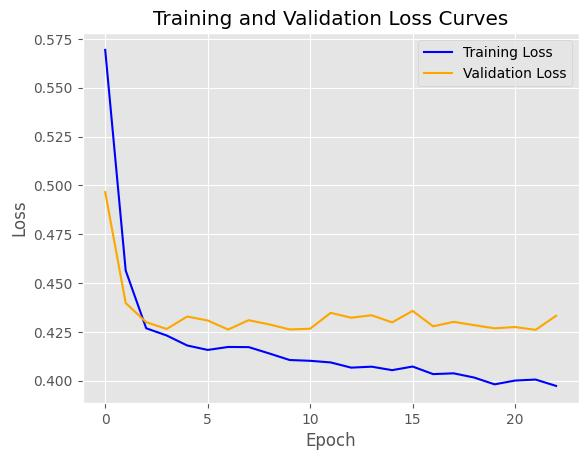
\includegraphics[width=1\linewidth]{Images/5.7.2.a.jpg}
    \caption{Training and Validation Loss Curves for Optimal Hyperparameters}
    \label{fig:enter-label}
\end{figure}

The loss curve shows the training loss (blue line) and validation loss (orange line) over 23 epochs. Initially, both losses decrease sharply, indicating that the model is learning quickly and fitting the training data well. However, the validation loss remains higher than the training loss, suggesting the model is not generalizing well to unseen data. As training continues, the losses level off, but the gap between the training loss and validation loss indicates potential overfitting. The fluctuating validation loss points to difficulty in generalizing. This suggests that regularization techniques or early stopping might be needed to improve the model’s generalization.

\subsubsection{Confusion Matrix}

\begin{figure}[hbt!]
    \centering
    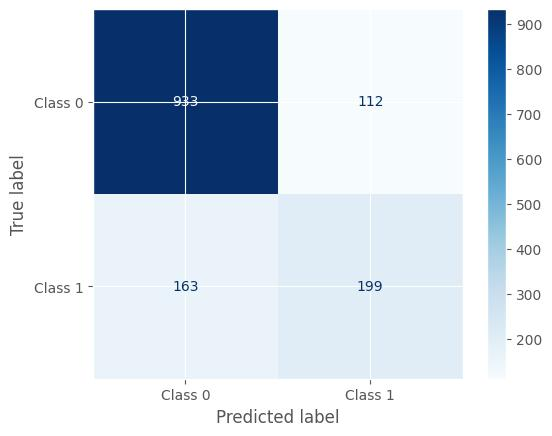
\includegraphics[width=1\linewidth]{Images/5.7.3.a.jpg}
    \caption{Confusion Matrix for Optimal Hyperparameters}
    \label{fig:enter-label}
\end{figure}

The confusion matrix shows that the model predicted 919 non-churning customers (True Negatives) and 195 churned customers (True Positives) correctly. However, it made 116 false positive errors, where it predicted churn when the customer did not churn, and 167 false negatives, where it failed to predict churn for customers who actually churned. While the model does a good job identifying non-churning customers, it misses many churn cases. Reducing these false negatives is essential to improving the model’s accuracy in predicting churn.

\subsubsection{ROC Curve and AUC Score}

\begin{figure}[hbt!]
    \centering
    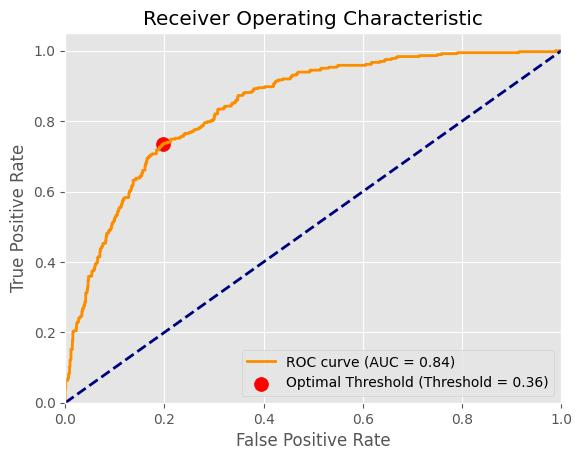
\includegraphics[width=1\linewidth]{Images/5.7.4.a.jpg}
    \caption{ROC Curve for Optimal Hyperparameters}
    \label{fig:enter-label}
\end{figure}

The ROC curve shows the model’s ability to distinguish between churned and non-churned customers. The AUC of 0.84 indicates the model is effective at differentiating between the two classes. The optimal threshold of 0.36, marked by the red dot on the curve, helps balance recall and precision. The curve is far from the diagonal line (representing random guessing), showing that the model is much better than random at identifying churn. The ROC curve confirms that the model is effective at minimizing errors while predicting churn.

\subsubsection{Precision-Recall Curve}

\begin{figure}[hbt!]
    \centering
    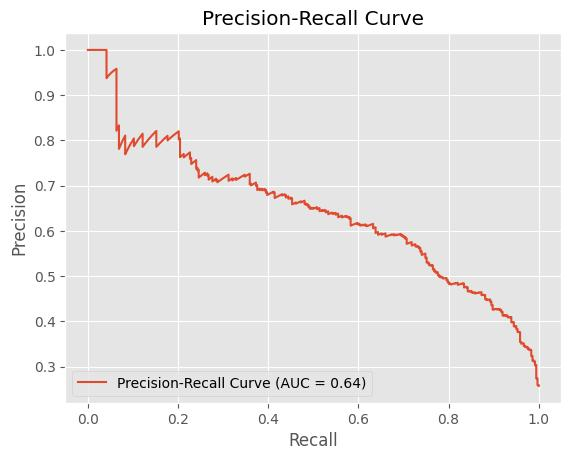
\includegraphics[width=1\linewidth]{Images/5.7.5.a.jpg}
    \caption{Precision-Recall Curve for Optimal Hyperparameters}
    \label{fig:enter-label}
\end{figure}

The Precision-Recall curve evaluates the model's performance with respect to churn cases (the positive class). The AUC of 0.64 shows that the model balances precision and recall moderately well. As recall increases (the model tries to capture more churn cases), precision drops significantly, which is typical when trying to capture as many churn cases as possible but at the cost of predicting more false positives. The trade-off between precision and recall is evident, suggesting that improving recall while reducing false positives could lead to better model performance. Overall, while the model is somewhat effective at churn prediction, there's room to improve, especially in minimizing false positives and increasing recall.

\subsection{Models Comparison}
When comparing the performance of the models trained with manual versus optimal hyperparameters, we can see that the optimal hyperparameters led to slight improvements in most performance metrics. The accuracy increased marginally from 79.89\% to 80.45\%, indicating a small but positive effect on the overall prediction accuracy. Precision also saw a modest boost, rising from 0.6270 to 0.6399, meaning the model became slightly more reliable in predicting churn. While recall showed a small improvement, moving from 0.5387 to 0.5497, it still remains relatively low, signaling a key area for further optimization. The F1 score also improved from 0.5795 to 0.5914, showing a better balance between precision and recall. The ROC AUC score increased slightly from 0.8351 to 0.8432, indicating the optimal hyperparameters helped the model better distinguish between churned and non-churned customers. Cross-validation results confirmed these improvements, with the model trained with optimal hyperparameters performing slightly better in terms of accuracy, precision, recall, F1 score, and ROC AUC. Despite the improvements, recall continues to be a challenge, and the models, while strong, could still be further fine-tuned to capture more churned customers.
